\documentclass{beamer}
\usetheme{Warsaw}

\usepackage[english]{babel}
% or whatever

\usepackage[latin1]{inputenc}
% or whatever

\usepackage{times}
\usepackage[T1]{fontenc}

\usepackage{graphicx}
\usepackage{color}
\usepackage{fancyvrb}

% Pygments syntax highlighting codes
<< pygments['pastie.tex'] >>


\title{Beamer Dexy Example}

\begin{document}

\begin{frame}
  \titlepage
\end{frame}

\begin{frame}[fragile]{Some Code}
Let's assign variables
<< d['code001.R|idio|r|pyg|l']['assign-variables'] >>
Now do multiplication
<< d['code001.R|idio|r|pyg|l']['multiply'] >>
\end{frame}

\begin{frame}[fragile]{A Graph}
Here's code for a graph:
<< d['code001.R|idio|r|pyg|l']['graph'] >>
And here's the graph:
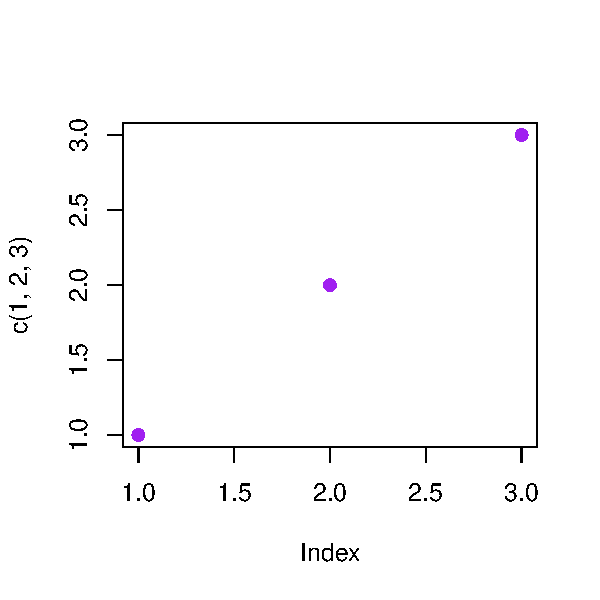
\includegraphics[width=4in]{plot.pdf}
\end{frame}


\end{document}


